\documentclass[conference]{IEEEtran}
\IEEEoverridecommandlockouts
\usepackage{cite}
\usepackage{amsmath,amssymb}
\usepackage{graphicx}
\usepackage{booktabs}
\usepackage{multirow}
\usepackage{textcomp}
\usepackage{xcolor}
\usepackage{url}
\usepackage[T1]{fontenc}

\newcommand{\ra}{$\rightarrow$}

\begin{document}

\title{What Is a Dysarthria Detector Listening To? Microphone, Speaker and Noise-Floor Shortcuts on TORGO}

% IEEE template order per author: name, department, organization, city/country, email.
% Add a department line (\textit{dept. name} \\) above the college if you want one.
\author{\IEEEauthorblockN{Abhiram Radhakrishnan}
\IEEEauthorblockA{\textit{Sri Sairam Engineering College}\\
Chennai, India \\
sec23am091@sairamtap.edu.in}
\and
\IEEEauthorblockN{Gengaraj P}
\IEEEauthorblockA{\textit{Sri Sairam Engineering College}\\
Chennai, India \\
sec23am057@sairamtap.edu.in}
\and
\IEEEauthorblockN{Praveen V}
\IEEEauthorblockA{\textit{Sri Sairam Engineering College}\\
Chennai, India \\
sec23am119@sairamtap.edu.in}
}

\maketitle

\begin{abstract}
Speech is an attractive signal for remote health monitoring because a phone can record it, and detectors for dysarthria often report accuracies above 90\% on public corpora. We ask how much of that performance belongs to the speech. On the TORGO corpus (15 speakers, 17,118 utterances, two microphones per session) we train two detectors, one on 88 interpretable eGeMAPS parameters with gradient-boosted trees and one on frozen WavLM embeddings with logistic regression, and then deliberately break the evaluation protocol in three ways to price each mistake. Splitting by utterance instead of by speaker lifts the area under the ROC curve (AUC) from 0.77 to 0.999. Letting the microphone differ between groups gives 0.999 as well, and the microphone itself can be identified from the same features with 99.5\% accuracy. A classifier that sees only the quietest tenth of each recording, which is mostly background, reaches an AUC of 0.86 on the far-field channel and beats both speech models there. With all three shortcuts closed, the honest figures are an AUC of 0.77 for eGeMAPS and 0.88 for WavLM, with wide speaker-level bootstrap intervals. The eGeMAPS model inverts when the microphone changes (AUC 0.14), because the level difference between patients and controls has opposite sign on the two channels. WavLM survives the change but identifies women with dysarthria far less reliably than men. Mild cases need tens of utterances before the decision stabilises. We close with a short reporting checklist for speech-based screening studies.
\end{abstract}

\begin{IEEEkeywords}
dysarthria, speech biomarkers, shortcut learning, data leakage, explainable AI, bias, telehealth, self-supervised speech models
\end{IEEEkeywords}

\section{Introduction}
Dysarthria is a motor speech disorder. It follows damage to the neural pathways that control the muscles of speech, and it appears in cerebral palsy, amyotrophic lateral sclerosis, Parkinson's disease, stroke and traumatic brain injury \cite{duffy2020,darley1969}. Speech becomes slow, imprecise, quiet or monotonous, depending on the subtype. In some conditions the changes are measurable early in the disease \cite{rusz2011}, and speech is about the cheapest clinical signal there is to collect: no consumables, no clinic visit, a microphone that the patient already owns. That is why speech keeps coming up in proposals for remote monitoring and telehealth screening \cite{moro2021}. If such monitoring is deployed, it will produce speech at a scale and from a variety of devices that no clinical corpus resembles, and the models applied to those streams will have been validated on the small laboratory collections that exist today.

The published numbers look ready for deployment. On the two standard English corpora, TORGO \cite{rudzicz2012} and UA-Speech \cite{kim2008}, reported accuracies for detection and severity classification are frequently above 90\% \cite{joshy2022,javanmardi2023,schu2023}. But both corpora are small (15 and 28 speakers) and neither was collected with machine-learning evaluation in mind. Schu \emph{et al.} \cite{schu2023} showed that several published classifiers do as well on the non-speech portions of these recordings as on the speech, which suggests that they partly separate recording sessions rather than speakers' speech. Medical imaging went through the same realisation a few years earlier, when pneumonia and COVID-19 classifiers turned out to be reading hospital-specific markers and patient positioning \cite{zech2018,degrave2021,roberts2021}. Geirhos \emph{et al.} call this \emph{shortcut learning} \cite{geirhos2020}: the model finds a rule that works on the benchmark and has nothing to do with the task.

Knowing that shortcuts exist is not the same as knowing their size. A practitioner who reads a 97\% figure cannot tell whether five points of it are artefact or forty. This paper tries to put numbers on that question for one corpus. We build two ordinary detectors on TORGO, evaluate them as carefully as we can, and then remove the safeguards one at a time. Each removal is a mistake that is easy to make by accident, and each has a measurable price.

Our contributions are the following.
\begin{itemize}
\item We quantify three shortcuts on the same data and models: speaker leakage through utterance-level splits, microphone identity aligned with the diagnosis, and group differences in the noise floor. Each one, alone, is enough to produce an AUC between 0.86 and 0.999.
\item We show that a detector built on interpretable acoustic parameters \emph{inverts} under a change of microphone (AUC 0.14), and we trace this to a level cue whose sign differs between the two TORGO channels. Frozen WavLM features do not invert, and training on both channels does not repair the eGeMAPS model.
\item We use SHAP not as a decoration but as an audit tool: it points at absolute loudness, and an ablation confirms that removing six level features takes the detector most of the way back to chance.
\item We report results per speaker, per severity band and per sex, with speaker-level bootstrap intervals. The sex gap for WavLM (AUC 0.96 for men, 0.69 for women) and the weak utterance-level accuracy on mild cases are both invisible in the pooled figure.
\item We distil the findings into six reporting items for studies that train health classifiers on small speech corpora.
\end{itemize}

We do not propose a new model. The detectors here are deliberately plain, and the honest numbers we end with are lower than most of the literature. We think that is the useful result.

\section{Related Work}
\subsection{Automatic dysarthria detection}
Early systems relied on hand-designed acoustic measures motivated by the clinical description of the disorder, such as jitter, shimmer, glottal parameters and rhythm metrics \cite{narendra2019,rusz2011}. Standardised parameter sets such as eGeMAPS \cite{eyben2016} made these comparable across studies. More recent work replaces them with representations from self-supervised models such as wav2vec~2.0 \cite{baevski2020}, HuBERT \cite{hsu2021} and WavLM \cite{chen2022}. Javanmardi \emph{et al.} \cite{javanmardi2023} used wav2vec~2.0 layers as features for detection and severity classification on UA-Speech, Yeo \emph{et al.} \cite{yeo2023} fine-tuned XLS-R with an auxiliary recognition task for severity classification, and Joshy and Rajan \cite{joshy2022} compared acoustic features with deep models on UA-Speech and TORGO. Wihlborg \emph{et al.} \cite{wihlborg2025} recently benchmarked 17 pretrained embedding systems on six dysarthria datasets and found that accuracy drops when the training and test datasets differ, which is the cross-corpus version of the effect we study inside a single corpus.

\subsection{Shortcuts and leakage in clinical machine learning}
Saeb \emph{et al.} \cite{saeb2017} showed that record-wise cross-validation, in which the same subject contributes to training and test folds, overestimates accuracy in clinical prediction, and argued for subject-wise splits. Kapoor and Narayanan \cite{kapoor2023} catalogued leakage across 17 fields and found it in hundreds of papers. In imaging, site and scanner effects have been shown to drive apparent diagnostic performance \cite{zech2018,degrave2021}, and a systematic review of COVID-19 imaging models found none fit for clinical use, largely because of such biases \cite{roberts2021}. Audio is not exempt: Coppock \emph{et al.} \cite{coppock2021} listed the same concerns for COVID-19 detection from cough and voice. Hidden stratification \cite{oakden2020} and unequal performance across demographic groups \cite{obermeyer2019} are the related fairness problems: a model can be good on average and poor on an identifiable subgroup.

\subsection{Recording conditions in dysarthric speech corpora}
The work closest to ours is Schu \emph{et al.} \cite{schu2023}, who separated speech from non-speech segments in UA-Speech and TORGO with a voice activity detector and found that most classifiers performed equally well or better on the non-speech part. We agree with their conclusion and build on it in four directions. First, we treat the three shortcuts separately so that each has its own price. Second, we use the fact that TORGO recorded two microphones to run a cross-channel test, which exposes a sign reversal that a single-channel analysis cannot see. Third, we include a frozen self-supervised model and find that it behaves differently from acoustic parameters under the channel change. Fourth, we carry the audit down to individual speakers, severity bands and sex.

\section{Data}
\subsection{The TORGO corpus}
TORGO \cite{rudzicz2012} contains speech from eight speakers with dysarthria (three women, five men) caused by cerebral palsy or amyotrophic lateral sclerosis, and from seven control speakers (three women, four men) matched roughly for age and sex. The material consists of single words, short sentences and non-speech oral tasks. Every session was recorded through a head-mounted microphone and through a microphone array placed in front of the speaker. The two channels do not cover the same set of utterances, and the split is uneven: speaker M05, for instance, has 475 head-microphone utterances and 119 array utterances, while F03 has 551 and 825.

Intelligibility of the dysarthric speakers was assessed with the Frenchay Dysarthria Assessment \cite{enderby1980}. We use the three-band grouping that is conventional for this corpus: F01, M01, M02 and M04 severe; F03 and M05 moderate; F04 and M03 mild.

\subsection{Filtering}
We built a manifest of all 17,633 audio files with a prompt directory and dropped an utterance only if its prompt was an instruction instead of text to be read (for example ``relax your mouth'') or if its duration was implausible (under 0.3~s or over 30~s). A missing transcript was not a reason to drop a file. That left 17,118 utterances and 14.3 hours of audio (Table~\ref{tab:corpus}). About 73\% of the retained prompts are single words, and the median utterance is 2.5~s long.

Any filter that removes more data from one group than the other is itself a possible confound, so we checked: instruction prompts account for 3.6\% of dysarthric and 2.2\% of control files, and the duration rule removes 0.7\% and 0\%.

\begin{table}[t]
\caption{Corpus after filtering}
\label{tab:corpus}
\centering
\begin{tabular}{lrrrr}
\toprule
 & \multicolumn{2}{c}{Head microphone} & \multicolumn{2}{c}{Array microphone}\\
\cmidrule(lr){2-3}\cmidrule(lr){4-5}
Group & Utterances & Hours & Utterances & Hours\\
\midrule
Dysarthric (8 speakers) & 2,848 & 2.85 & 3,065 & 2.85\\
Control (7 speakers) & 5,097 & 3.77 & 6,108 & 4.82\\
\midrule
Total & 7,945 & 6.62 & 9,173 & 7.67\\
\bottomrule
\end{tabular}
\end{table}

\section{Methods}
\subsection{Two detectors}
\subsubsection{eGeMAPS with gradient-boosted trees}
We extract the 88 functionals of eGeMAPSv02 \cite{eyben2016} with openSMILE \cite{eyben2010}. They summarise pitch, loudness, jitter, shimmer, harmonics-to-noise ratio, formants, spectral slope, MFCCs 1--4 and a few timing statistics over the whole utterance. The classifier is XGBoost \cite{chen2016} with 400 trees of depth 4, learning rate 0.05, row subsampling 0.8, column subsampling 0.6, an $\ell_2$ penalty of 2 and a minimum child weight of 5. We fixed these values once, before looking at test results, and did not tune them; with 15 speakers there is no room for a validation set that would not itself leak.

\subsubsection{Frozen WavLM with logistic regression}
We pass each peak-normalised waveform, truncated to 12~s, through \texttt{wavlm-base-plus} \cite{chen2022} and take the last hidden layer. Frames are pooled over time into a mean and a standard deviation, giving 1,536 dimensions per utterance. The encoder is never updated. Fine-tuning 94 million parameters on 14 training speakers would invite the model to memorise them, and a frozen encoder also keeps the comparison with eGeMAPS about the features and not the training recipe. On top we fit an $\ell_2$-regularised logistic regression ($C=0.1$) on standardised inputs. A one-hidden-layer perceptron (256 units) is included as a check that the linear model is not leaving much behind.

\subsection{Evaluation protocol}
\label{sec:protocol}
Every reported number, unless we say otherwise, comes from leave-one-speaker-out (LOSO) cross-validation: 15 folds, each training on 14 speakers and testing on all utterances of the fifteenth. Nothing from the held-out speaker reaches training, including the statistics of the feature scaler.

Speakers contribute between 123 and 1,091 head-microphone utterances. To stop the talkative ones from defining the decision boundary we weight training utterances so that every speaker carries the same total weight, and then rescale so that the two classes do as well.

A held-out fold contains one class only, so per-fold AUC is undefined. We pool the out-of-fold probabilities and report accuracy, balanced accuracy, sensitivity, specificity and AUC at the utterance level. A screening tool, however, judges a person and not an utterance. We therefore also report how many of the 15 speakers are classified correctly when their utterance probabilities are averaged and thresholded at 0.5, and the AUC of those 15 speaker scores.

\subsubsection{Uncertainty}
Utterances from one speaker are far from independent, so intervals computed over utterances would be much too narrow. We use a cluster bootstrap \cite{efron1993}: speakers are resampled with replacement within each group, 2,000 times, and all utterances of a drawn speaker travel together. For speaker counts we give exact binomial intervals. Model comparisons use the same bootstrap draws for both models, which makes them paired.

\subsection{The audit}
\label{sec:audit}
The primary protocol fixes the head microphone for both groups. Around it we arrange the following experiments. All of them keep the LOSO structure except the one that tests it.

\begin{enumerate}
\item \emph{Speaker leakage.} The same data and model, but with a 15-fold split over utterances, stratified by speaker. Every test utterance then has several hundred siblings from the same person in training.
\item \emph{Channel probe.} The label is replaced by the microphone (head or array). If held-out speakers' microphones can be identified from the features, the features carry channel information that a detector could exploit.
\item \emph{Aligned channel.} Dysarthric speakers are taken from one microphone and controls from the other, and then the reverse. This is the error an inattentive data loader would make, since TORGO stores both channels side by side.
\item \emph{Cross-channel transfer.} Train on one microphone, test the held-out speaker on the other.
\item \emph{Pooled training.} Train on both microphones and test on each. This is the obvious cheap remedy, in the spirit of multi-condition training.
\item \emph{Matched material.} Restrict the data to prompts that at least one speaker of each group read (6,407 head-microphone utterances), to check that the detector is not reading the script.
\item \emph{Quiet-frame probe.} For every utterance we compute a 40-band log-mel spectrogram (25~ms windows, 10~ms hop), sort frames by energy, and keep the quietest 10\%. Their per-band mean and standard deviation form an 80-dimensional descriptor that contains leading and trailing silence, pauses and background, and very little speech. A second version subtracts each frame's mean log energy, leaving only the spectral shape of the noise. For reference, the same statistics are computed on the loudest half of the frames.
\item \emph{Level ablation.} Guided by the explanation in Section~\ref{sec:shap}, we remove the six eGeMAPS parameters that measure absolute level (mean loudness, its three percentiles and percentile range, and equivalent sound level) and keep scale-free ones such as the coefficient of variation of loudness.
\end{enumerate}

\subsection{Explanation}
For the tree model we compute SHAP values with the exact tree algorithm \cite{lundberg2017,lundberg2020}. The model is refitted in every LOSO fold and values are computed only for the held-out speaker, so the attribution describes behaviour on unseen people. We rank features by mean absolute SHAP value over all 7,945 held-out utterances.

\subsection{Implementation}
The pipeline is written in Python with scikit-learn \cite{pedregosa2011}. It runs on a 16-core CPU: about 20 minutes for eGeMAPS, 2.5 hours for WavLM extraction, and minutes for each LOSO run. Result tables are generated by code from stored predictions. A unit test asserts that no held-out speaker occurs in its own training set. Code and per-utterance predictions are available from the authors on request; the audio must be obtained from the corpus maintainers.

\section{Results}
\subsection{The careful protocol}
Table~\ref{tab:main} gives the head-microphone results. Frozen WavLM with a linear classifier reaches an AUC of 0.883 and classifies 14 of 15 speakers correctly (exact 95\% interval for the proportion: 0.68 to 1.00). eGeMAPS with XGBoost reaches 0.765 and 13 of 15 (0.60 to 0.98). The perceptron on WavLM features is no better than the linear model. Restricting to shared prompts changes neither model by more than 0.01 AUC, so the script is not what is being detected.

The intervals deserve as much attention as the point estimates. With 15 speakers, the 95\% interval for the eGeMAPS AUC runs from 0.57 to 0.92. The gap between WavLM and eGeMAPS is 0.118 AUC with a paired interval of $[-0.02, 0.30]$; 5\% of bootstrap draws favour eGeMAPS. We believe WavLM is the better feature set here, but 15 speakers cannot establish it at the conventional level. Repeating the XGBoost run with five seeds moved its AUC only between 0.762 and 0.771, and the speaker count stayed at 13, so the uncertainty comes from who is in the corpus, not from the optimiser.

The speaker-level AUC is 0.98 for WavLM and 0.84 for eGeMAPS. Averaging over a session helps both models, WavLM more.

\begin{table*}[t]
\caption{Leave-one-speaker-out results. Brackets give 95\% speaker-level bootstrap intervals. eGeMAPS features are missing for two array-microphone files.}
\label{tab:main}
\centering
\begin{tabular}{llrcccccc}
\toprule
Features + classifier & Condition & Utt. & Acc. & Bal. acc. & AUC & Sens. & Spec. & Speakers\\
\midrule
\multicolumn{9}{l}{\emph{Head microphone (primary protocol)}}\\
eGeMAPS (88) + XGBoost & all prompts & 7,945 & 0.720 & 0.716 [0.57, 0.85] & 0.765 [0.57, 0.92] & 0.703 & 0.730 & 13/15\\
eGeMAPS (88) + XGBoost & shared prompts & 6,407 & 0.729 & 0.732 [0.58, 0.87] & 0.771 [0.58, 0.93] & 0.756 & 0.709 & 13/15\\
eGeMAPS (82) + XGBoost & no level features & 7,945 & 0.575 & 0.572 [0.42, 0.72] & 0.589 [0.38, 0.78] & 0.561 & 0.583 & 10/15\\
WavLM (1,536) + log. reg. & all prompts & 7,945 & \textbf{0.822} & \textbf{0.812} [0.70, 0.92] & \textbf{0.883} [0.77, 0.98] & 0.775 & 0.848 & \textbf{14/15}\\
WavLM (1,536) + log. reg. & shared prompts & 6,407 & 0.805 & 0.802 [0.70, 0.91] & 0.875 [0.76, 0.98] & 0.777 & 0.826 & 14/15\\
WavLM (1,536) + MLP & all prompts & 7,945 & 0.803 & 0.798 [0.68, 0.91] & 0.870 [0.74, 0.98] & 0.779 & 0.817 & 13/15\\
\midrule
\multicolumn{9}{l}{\emph{Array microphone (replication)}}\\
eGeMAPS (88) + XGBoost & all prompts & 9,171 & 0.556 & 0.556 [0.37, 0.77] & 0.590 [0.33, 0.91] & 0.556 & 0.557 & 10/15\\
WavLM (1,536) + log. reg. & all prompts & 9,173 & 0.695 & 0.668 [0.53, 0.82] & 0.729 [0.56, 0.91] & 0.590 & 0.747 & 10/15\\
\bottomrule
\end{tabular}
\end{table*}

\subsection{What each shortcut is worth}
Fig.~\ref{fig:audit} and Table~\ref{tab:audit} summarise the audit.

\begin{figure*}[t]
\centering
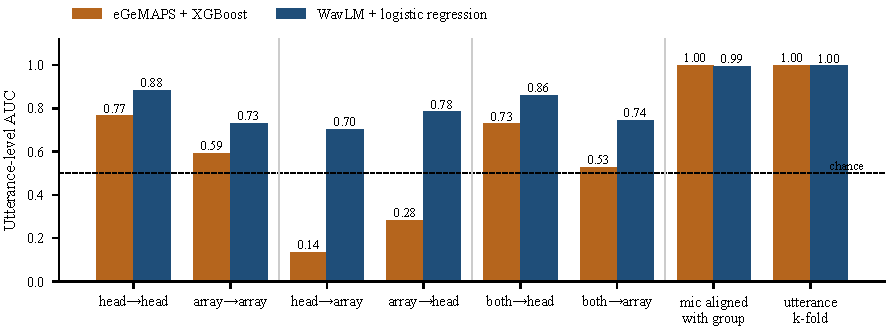
\includegraphics[width=0.95\textwidth]{figs/audit.pdf}
\caption{Utterance-level AUC under each evaluation condition. ``a\ra b'' means trained on microphone a and tested on microphone b, with the test speaker held out. The two rightmost conditions are the protocol errors: microphone aligned with diagnosis, and folds drawn over utterances so that speakers repeat across training and test.}
\label{fig:audit}
\end{figure*}

\subsubsection{Speaker leakage}
With utterance-level folds the eGeMAPS model scores an AUC of 0.999 and an accuracy of 99.1\%; WavLM scores 0.995 and 97.4\%. Nothing else changed. The entire distance between the low seventies and the high nineties, for the acoustic model, is the model recognising people it has already heard. This matches what Saeb \emph{et al.} \cite{saeb2017} found for wearable-sensor data, and on a corpus with 15 speakers and hundreds of utterances each the effect is close to total.

\subsubsection{Microphone identity}
The microphone can be read from eGeMAPS features of held-out speakers with 99.5\% accuracy and from WavLM embeddings with 98.3\%. When the microphone is aligned with the diagnosis, both detectors look nearly perfect under a correct LOSO split: an AUC of 0.999 and all 15 speakers correct for eGeMAPS, 0.994 for WavLM. Speaker-independent evaluation alone does not protect against this. The model has learnt to tell two microphones apart and gets credited with a diagnosis.

Removing the level features does not close this hole either. The 82-feature model still identifies the microphone with 99.7\% accuracy, so the channel signature is spread across the spectral parameters.

\subsubsection{Changing the channel}
An eGeMAPS model trained on the head microphone and tested on the array gives an AUC of 0.135. That is not noise around 0.5. The model's ranking is mostly \emph{reversed}: it assigns higher probabilities to controls than to patients. The other direction gives 0.283. WavLM does not show this. It loses ground (0.702 from head to array) but keeps its orientation, and from array to head it scores 0.783, higher than the array-only result of 0.729. The array test data seem to be the hard part, more than the array training data.

The reversal has a simple origin. For each speaker we took the median over utterances of eGeMAPS median loudness. On the head microphone the dysarthric speakers are quieter than the controls (group medians 0.15 and 0.30, Mann--Whitney $p=0.006$ over the 15 speakers). On the array microphone, in the same sessions, they are louder (0.18 against 0.15, $p=0.006$), and their equivalent sound level is about 11~dB higher. A level difference that changes sign with the microphone cannot be purely a property of the speakers' voices. Something in the set-up, such as gain or the distance to the array, must have differed between the groups on at least one of the channels. A tree model that learnt ``quiet means dysarthric'' on one channel applies the rule on the other and gets the wrong answer with confidence.

Training on both channels at once is not a remedy for the acoustic model: its AUC is 0.727 on head-microphone tests and 0.526 on array tests. For WavLM the pooled model is about as good as the matched ones (0.859 and 0.744).

\begin{table}[t]
\caption{Audit conditions. AUC with accuracy in parentheses.}
\label{tab:audit}
\centering
\setlength{\tabcolsep}{3.5pt}
\begin{tabular}{lccc}
\toprule
 & eGeMAPS & eGeMAPS & WavLM\\
Condition & + XGBoost & no level & + log. reg.\\
\midrule
\multicolumn{4}{l}{\emph{LOSO, one microphone}}\\
head\ra head & 0.765 (0.72) & 0.589 (0.57) & 0.883 (0.82)\\
array\ra array & 0.590 (0.56) & 0.593 (0.59) & 0.729 (0.69)\\
\multicolumn{4}{l}{\emph{LOSO, microphone changes}}\\
head\ra array & 0.135 (0.23) & 0.286 (0.31) & 0.702 (0.72)\\
array\ra head & 0.283 (0.25) & 0.403 (0.34) & 0.783 (0.66)\\
both\ra head & 0.727 (0.72) & 0.607 (0.61) & 0.859 (0.80)\\
both\ra array & 0.526 (0.54) & 0.541 (0.55) & 0.744 (0.70)\\
\multicolumn{4}{l}{\emph{Protocol errors}}\\
dys.\ head, ctrl.\ array & 0.999 (0.97) & 0.999 (0.98) & 0.994 (0.97)\\
dys.\ array, ctrl.\ head & 1.000 (0.99) & 1.000 (0.99) & 0.997 (0.98)\\
utterance 15-fold, head & 0.999 (0.99) & -- & 0.995 (0.97)\\
\midrule
Microphone probe & 1.000 (0.995) & 1.000 (0.997) & 0.998 (0.98)\\
\bottomrule
\end{tabular}
\end{table}

\subsubsection{The noise floor}
Table~\ref{tab:quiet} gives the quiet-frame probe. On the head microphone, a classifier that sees only the quietest tenth of each recording reaches an AUC of 0.67 to 0.70 and, with XGBoost, classifies 13 of 15 speakers correctly. That is the same speaker count as the full eGeMAPS model. On the array microphone the quiet frames give 0.859 and 14 of 15 speakers, which is better than either speech-based detector on that channel (0.590 and 0.729).

When the overall level is removed from the quiet frames and only the spectral shape remains, the head-microphone result falls to chance for the linear model (0.48), while the array result stays near 0.69. So on the head microphone the usable non-speech information is mostly \emph{level}, and on the array there is in addition a difference in the colour of the background. The loudest half of the frames, where the speech is, carries less group information in this crude representation than the quietest tenth.

We do not want to overread this. Quiet frames in dysarthric speech are not pure background: breathy onsets, weak consonants and audible breathing can land there, and reduced vocal intensity is a clinical sign in its own right \cite{duffy2020}. But the array result, taken together with the sign reversal above, is hard to explain by physiology alone.

\begin{table}[t]
\caption{Detecting dysarthria from the quietest 10\% of frames (LOSO). AUC with correctly classified speakers.}
\label{tab:quiet}
\centering
\setlength{\tabcolsep}{4pt}
\begin{tabular}{llcc}
\toprule
Frames used & Classifier & Head mic. & Array mic.\\
\midrule
Quietest 10\% & log. reg. & 0.674 (11/15) & 0.859 (14/15)\\
Quietest 10\% & XGBoost & 0.703 (13/15) & 0.735 (12/15)\\
Quietest 10\%, shape only & log. reg. & 0.479 (8/15) & 0.687 (11/15)\\
Quietest 10\%, shape only & XGBoost & 0.636 (10/15) & 0.690 (12/15)\\
Loudest 50\% & log. reg. & 0.598 (11/15) & 0.625 (12/15)\\
Loudest 50\% & XGBoost & 0.654 (11/15) & 0.549 (11/15)\\
\midrule
\multicolumn{2}{l}{eGeMAPS + XGBoost (Table~\ref{tab:main})} & 0.765 (13/15) & 0.590 (10/15)\\
\multicolumn{2}{l}{WavLM + log. reg. (Table~\ref{tab:main})} & 0.883 (14/15) & 0.729 (10/15)\\
\bottomrule
\end{tabular}
\end{table}

\subsection{What the acoustic model uses}
\label{sec:shap}
Fig.~\ref{fig:shap} shows the SHAP ranking on held-out speakers. One parameter dominates: the 20th percentile of loudness, which is the loudness of the quiet parts of the utterance. Its mean absolute contribution (2.0 in log-odds) is almost three times that of the next feature. Median loudness and equivalent sound level are also in the top six. Behind them come parameters with a recognisable clinical reading: H1--H2, which relates to breathiness; the variability of pitch; the variability and mean length of unvoiced segments, a proxy for pausing; and, just outside the twelve shown, the rate of loudness peaks, a proxy for syllable rate. Slow rate, irregular pauses, monopitch and breathy voice are textbook perceptual features of dysarthria \cite{darley1969}.

\begin{figure}[t]
\centering
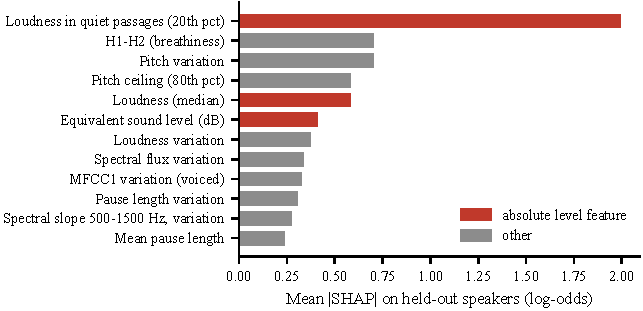
\includegraphics[width=\columnwidth]{figs/shap.pdf}
\caption{The twelve most influential eGeMAPS parameters for the XGBoost detector, computed on held-out speakers only.}
\label{fig:shap}
\end{figure}

The explanation is therefore half reassuring. The model does attend to things a speech-language pathologist would name. But its single most important input is the level of the quiet passages, and Table~\ref{tab:quiet} has just shown that the quiet passages alone carry group information. The level ablation makes the dependence concrete: without the six absolute level features, the AUC drops from 0.765 to 0.589 (difference 0.176, paired interval $[0.08, 0.29]$) and three more speakers are misclassified, including both mild cases. On the head microphone, most of what this detector knows is how loud the recording is.

Whether that loudness is hypophonia or gain cannot be settled from TORGO. The sign reversal on the array says some of it is set-up. For a telehealth application the distinction hardly matters, because absolute level is not something a patient's phone will reproduce in any case.

\subsection{Who is misclassified}
\subsubsection{Severity}
Table~\ref{tab:sev} breaks the head-microphone results down by severity. Severe dysarthria is detected almost perfectly by both models. For WavLM the mild band is the weakest at the utterance level (0.568, not far above a coin), and both mild speakers are still classified correctly as people only because their mean probability sits just above the threshold (0.57 and 0.56). For eGeMAPS the moderate band is the weakest.

That disagreement between models is a warning about the table itself. Each band has two to four people. The ``moderate'' row is F03 and M05 and nothing else. Fig.~\ref{fig:speakers} shows the individual speakers. F03 is read as a control by every detector in Table~\ref{tab:main}, on both microphones. MC04, a control, receives a mean probability of 0.96 from the eGeMAPS model and 0.10 from WavLM. His head-microphone recordings have the lowest quiet-passage loudness among the controls, and the model that relies on level is the one that is fooled.

\begin{table}[t]
\caption{Head-microphone results by severity band}
\label{tab:sev}
\centering
\setlength{\tabcolsep}{4pt}
\begin{tabular}{lrrcccc}
\toprule
 & & & \multicolumn{2}{c}{eGeMAPS + XGB} & \multicolumn{2}{c}{WavLM + LR}\\
\cmidrule(lr){4-5}\cmidrule(lr){6-7}
Band & Spk. & Utt. & Utt. acc. & Spk. & Utt. acc. & Spk.\\
\midrule
Control & 7 & 5,097 & 0.730 & 6/7 & 0.848 & 7/7\\
Mild & 2 & 651 & 0.751 & 2/2 & 0.568 & 2/2\\
Moderate & 2 & 1,026 & 0.421 & 1/2 & 0.669 & 1/2\\
Severe & 4 & 1,171 & 0.923 & 4/4 & 0.984 & 4/4\\
\bottomrule
\end{tabular}
\end{table}

\begin{figure}[t]
\centering
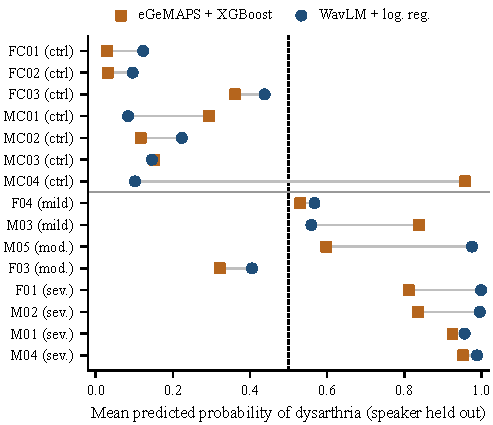
\includegraphics[width=\columnwidth]{figs/speakers.pdf}
\caption{Mean out-of-fold probability for each speaker (head microphone). Controls should fall left of the dashed line and dysarthric speakers right of it.}
\label{fig:speakers}
\end{figure}

\subsubsection{Sex}
Split by sex, the WavLM detector has an AUC of 0.961 on the nine men and 0.687 on the six women; sensitivity is 0.89 for men and 0.53 for women. The eGeMAPS model shows a smaller gap in AUC (0.795 and 0.718) but a similar one in sensitivity (0.82 and 0.45). TORGO has only three women with dysarthria, one in each severity band, and one of them is F03, so we cannot separate an effect of sex from an effect of these three individuals. We report the gap because a pooled AUC of 0.88 gives no hint of it, and because a screening tool that misses half of the affected women would be a clinical and an ethical problem regardless of its average \cite{oakden2020,obermeyer2019}.

\subsection{How long must the system listen?}
A screening tool will hear more than one utterance. For each speaker we drew $k$ held-out utterances at random, averaged their probabilities and repeated this 2,000 times (Fig.~\ref{fig:listen}). For WavLM, control speakers are right 86\% of the time from one utterance and 96\% from ten. Mild speakers are right 57\% of the time from one utterance, 69\% from ten and 89\% from fifty. A single word is close to uninformative for a mild case; a session of several dozen short utterances is not.

Averaging does not rescue everyone. The moderate curve for WavLM \emph{falls} with $k$, from 0.69 to 0.50. This is the average of M05, who is always detected, and F03, whose mean probability is 0.41: the more of her speech the system hears, the more certain it becomes of the wrong answer. Longer listening reduces variance and leaves bias where it was.

\begin{figure}[t]
\centering
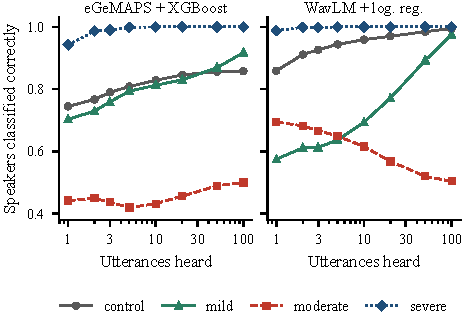
\includegraphics[width=\columnwidth]{figs/listening.pdf}
\caption{Probability of classifying a held-out speaker correctly after averaging over $k$ randomly drawn utterances, by severity band (head microphone, 2,000 draws per point).}
\label{fig:listen}
\end{figure}

\section{Discussion}
\subsection{Reading published numbers}
On this corpus, three different mistakes each produce a near-perfect detector: mixing a speaker's utterances across folds, mixing microphones across groups, and, on the array channel, simply listening to the background. A paper that reports 97\% on TORGO without stating the split unit and the channel has not given the reader enough to know which of these it measured. We are not claiming that any particular prior result is wrong. Our claim is narrower: the high figures are reachable without modelling dysarthria at all, so they are weak evidence that dysarthria was modelled.

The careful figure for the better of our two models, an AUC of 0.88 with an interval from 0.77 to 0.98, is still not a statement about patients in general. It describes eight people with cerebral palsy or ALS and seven controls, reading prompts in a laboratory in Toronto.

\subsection{Interpretable features were the fragile ones}
We expected the interpretable model to be the safer choice. In one respect it was: because eGeMAPS parameters have names, SHAP could tell us that the detector leaned on loudness, and we could test that. The WavLM model offers no such handle. Yet the interpretable model was also the one that inverted under a channel change, was fooled by a quiet control speaker, and could not be repaired by pooled training. Frozen WavLM embeddings of peak-normalised audio degraded but did not invert. Large-scale pretraining on varied audio appears to buy some invariance to level and channel that a fixed set of functionals does not have. Even so, the microphone remains almost perfectly decodable from WavLM embeddings, so the model is robust in this case without being blind to the channel. Interpretability helped us find the problem. It did not prevent it.

\subsection{Implications for telehealth}
In remote monitoring, the microphone is never controlled. Patients use different phones, hold them at different distances and sit in different rooms. The cross-channel experiment is a small rehearsal of that situation with only two devices, and one of our detectors failed it completely. Two practical points follow. A detector meant for the field should be tested on at least one recording condition that it was not trained on, and features that measure absolute level should either be calibrated or left out, with the loss in accuracy accepted and reported. And since mild cases only become detectable after tens of utterances, a screening protocol should be designed around a short session, with the decision deferred until enough speech has been heard.

\subsection{A reporting checklist}
Reporting guidelines such as TRIPOD \cite{collins2015} cover clinical prediction models in general. For small speech corpora we suggest six additional items, each of which changed a conclusion in this study.
\begin{enumerate}
\item \emph{State the split unit.} Folds must be disjoint in speakers, including for scalers and any other fitted preprocessing. Report the utterance-level split as a reference if you like, labelled as such.
\item \emph{State the recording channel for each group} and run a channel probe. If the features can identify the channel or session, say so.
\item \emph{Run a non-speech baseline.} A classifier on silence or low-energy frames gives a floor that the speech model has to beat.
\item \emph{Test on a held-out recording condition} when the corpus offers more than one.
\item \emph{Report per speaker and per subgroup}, with intervals resampled over speakers. With fewer than a few dozen speakers, the individual table is the result.
\item \emph{Attribute, then ablate.} If an explanation method ranks a feature that the recording set-up could influence, remove it and report what is left.
\end{enumerate}

\subsection{Limitations}
This is an audit of a single corpus with 15 speakers. The intervals are wide, and several comparisons we find suggestive (WavLM against eGeMAPS, men against women) do not reach conventional significance. The quiet-frame selection is an energy rule and not a voice activity detector, so some low-level speech is included. We did not tune hyperparameters, and tuned models might do somewhat better under the careful protocol; they would also do better under the flawed ones. We used one self-supervised encoder and its last layer only, although other layers are known to suit paralinguistic tasks better \cite{javanmardi2023}. Our severity labels follow convention and compress a multi-dimensional clinical assessment into three bands. Finally, we could not determine \emph{why} the level difference reverses between microphones, because the session set-up is not documented at that level of detail; we can only show that it does.

\section{Conclusion}
On TORGO, a dysarthria detector can reach an AUC of 0.999 by recognising speakers, 0.999 by recognising microphones and 0.86 by listening to the quietest frames. With those routes closed, the same models reach 0.77 and 0.88 and classify 13 and 14 of 15 speakers, with intervals that reflect how few people that is. The acoustic model depends on recording level strongly enough to invert when the microphone changes. The self-supervised model is sturdier, but it detects women less reliably than men and needs a session's worth of speech for mild cases. None of this argues against speech as a clinical signal. It argues that, for corpora of this size, the evaluation protocol decides the reported number more than the model does, and that the protocol should be described with the same care as the architecture. The next step is to repeat the audit on corpora with documented multi-device recordings, where the level question can actually be answered.

\section*{Ethical Considerations}
This study uses only the publicly distributed TORGO corpus under its academic licence; no new data were collected and no participant can be identified from the reported results. The detectors described are research artefacts. They have not been validated for clinical use and must not inform decisions about any individual's care.

% ---------------------------------------------------------------------------
% IEEE policy requires AI-generated text to be disclosed in the acknowledgments.
% Uncomment and adapt before submission.
% ---------------------------------------------------------------------------
%\section*{Acknowledgment}
%Portions of the text, analysis code and figures in this paper were drafted with the assistance of Claude (Anthropic) and were reviewed and verified by the author, who takes full responsibility for the content.

\begin{thebibliography}{00}
\bibitem{duffy2020} J. R. Duffy, \emph{Motor Speech Disorders: Substrates, Differential Diagnosis, and Management}, 4th ed. St. Louis, MO, USA: Elsevier, 2020.
\bibitem{darley1969} F. L. Darley, A. E. Aronson, and J. R. Brown, ``Differential diagnostic patterns of dysarthria,'' \emph{J. Speech Hear. Res.}, vol. 12, no. 2, pp. 246--269, 1969.
\bibitem{rusz2011} J. Rusz, R. Cmejla, H. Ruzickova, and E. Ruzicka, ``Quantitative acoustic measurements for characterization of speech and voice disorders in early untreated Parkinson's disease,'' \emph{J. Acoust. Soc. Amer.}, vol. 129, no. 1, pp. 350--367, 2011.
\bibitem{moro2021} L. Moro-Velazquez, J. A. Gomez-Garcia, J. D. Arias-Londo\~no, N. Dehak, and J. I. Godino-Llorente, ``Advances in Parkinson's disease detection and assessment using voice and speech: A review of the articulatory and phonatory aspects,'' \emph{Biomed. Signal Process. Control}, vol. 66, Art. no. 102418, 2021.
\bibitem{rudzicz2012} F. Rudzicz, A. K. Namasivayam, and T. Wolff, ``The TORGO database of acoustic and articulatory speech from speakers with dysarthria,'' \emph{Lang. Resour. Eval.}, vol. 46, no. 4, pp. 523--541, 2012.
\bibitem{kim2008} H. Kim \emph{et al.}, ``Dysarthric speech database for universal access research,'' in \emph{Proc. Interspeech}, 2008, pp. 1741--1744.
\bibitem{joshy2022} A. A. Joshy and R. Rajan, ``Automated dysarthria severity classification: A study on acoustic features and deep learning techniques,'' \emph{IEEE Trans. Neural Syst. Rehabil. Eng.}, vol. 30, pp. 1147--1157, 2022.
\bibitem{javanmardi2023} F. Javanmardi, S. Tirronen, M. Kodali, S. R. Kadiri, and P. Alku, ``Wav2vec-based detection and severity level classification of dysarthria from speech,'' in \emph{Proc. IEEE Int. Conf. Acoust., Speech, Signal Process. (ICASSP)}, 2023, pp. 1--5.
\bibitem{schu2023} G. Schu, P. Janbakhshi, and I. Kodrasi, ``On using the UA-Speech and TORGO databases to validate automatic dysarthric speech classification approaches,'' in \emph{Proc. IEEE Int. Conf. Acoust., Speech, Signal Process. (ICASSP)}, 2023, pp. 1--5.
\bibitem{zech2018} J. R. Zech, M. A. Badgeley, M. Liu, A. B. Costa, J. J. Titano, and E. K. Oermann, ``Variable generalization performance of a deep learning model to detect pneumonia in chest radiographs: A cross-sectional study,'' \emph{PLoS Med.}, vol. 15, no. 11, Art. no. e1002683, 2018.
\bibitem{degrave2021} A. J. DeGrave, J. D. Janizek, and S.-I. Lee, ``AI for radiographic COVID-19 detection selects shortcuts over signal,'' \emph{Nature Mach. Intell.}, vol. 3, no. 7, pp. 610--619, 2021.
\bibitem{roberts2021} M. Roberts \emph{et al.}, ``Common pitfalls and recommendations for using machine learning to detect and prognosticate for COVID-19 using chest radiographs and CT scans,'' \emph{Nature Mach. Intell.}, vol. 3, no. 3, pp. 199--217, 2021.
\bibitem{geirhos2020} R. Geirhos \emph{et al.}, ``Shortcut learning in deep neural networks,'' \emph{Nature Mach. Intell.}, vol. 2, no. 11, pp. 665--673, 2020.
\bibitem{narendra2019} N. P. Narendra and P. Alku, ``Dysarthric speech classification from coded telephone speech using glottal features,'' \emph{Speech Commun.}, vol. 110, pp. 47--55, 2019.
\bibitem{eyben2016} F. Eyben \emph{et al.}, ``The Geneva minimalistic acoustic parameter set (GeMAPS) for voice research and affective computing,'' \emph{IEEE Trans. Affect. Comput.}, vol. 7, no. 2, pp. 190--202, 2016.
\bibitem{baevski2020} A. Baevski, H. Zhou, A. Mohamed, and M. Auli, ``wav2vec 2.0: A framework for self-supervised learning of speech representations,'' in \emph{Adv. Neural Inf. Process. Syst.}, vol. 33, 2020.
\bibitem{hsu2021} W.-N. Hsu, B. Bolte, Y.-H. H. Tsai, K. Lakhotia, R. Salakhutdinov, and A. Mohamed, ``HuBERT: Self-supervised speech representation learning by masked prediction of hidden units,'' \emph{IEEE/ACM Trans. Audio, Speech, Lang. Process.}, vol. 29, pp. 3451--3460, 2021.
\bibitem{chen2022} S. Chen \emph{et al.}, ``WavLM: Large-scale self-supervised pre-training for full stack speech processing,'' \emph{IEEE J. Sel. Topics Signal Process.}, vol. 16, no. 6, pp. 1505--1518, 2022.
\bibitem{yeo2023} E. J. Yeo, K. Choi, S. Kim, and M. Chung, ``Automatic severity classification of dysarthric speech by using self-supervised model with multi-task learning,'' in \emph{Proc. IEEE Int. Conf. Acoust., Speech, Signal Process. (ICASSP)}, 2023, pp. 1--5.
\bibitem{wihlborg2025} L. Wihlborg \emph{et al.}, ``Evaluating pretrained speech embedding systems for dysarthria detection across heterogenous datasets,'' arXiv preprint arXiv:2509.19946, 2025.
\bibitem{saeb2017} S. Saeb, L. Lonini, A. Jayaraman, D. C. Mohr, and K. P. Kording, ``The need to approximate the use-case in clinical machine learning,'' \emph{GigaScience}, vol. 6, no. 5, Art. no. gix019, 2017.
\bibitem{kapoor2023} S. Kapoor and A. Narayanan, ``Leakage and the reproducibility crisis in machine-learning-based science,'' \emph{Patterns}, vol. 4, no. 9, Art. no. 100804, 2023.
\bibitem{coppock2021} H. Coppock, L. Jones, I. Kiskin, and B. Schuller, ``COVID-19 detection from audio: Seven grains of salt,'' \emph{Lancet Digit. Health}, vol. 3, no. 9, pp. e537--e538, 2021.
\bibitem{oakden2020} L. Oakden-Rayner, J. Dunnmon, G. Carneiro, and C. R\'e, ``Hidden stratification causes clinically meaningful failures in machine learning for medical imaging,'' in \emph{Proc. ACM Conf. Health, Inference, Learn. (CHIL)}, 2020, pp. 151--159.
\bibitem{obermeyer2019} Z. Obermeyer, B. Powers, C. Vogeli, and S. Mullainathan, ``Dissecting racial bias in an algorithm used to manage the health of populations,'' \emph{Science}, vol. 366, no. 6464, pp. 447--453, 2019.
\bibitem{enderby1980} P. Enderby, ``Frenchay dysarthria assessment,'' \emph{Brit. J. Disord. Commun.}, vol. 15, no. 3, pp. 165--173, 1980.
\bibitem{eyben2010} F. Eyben, M. W\"ollmer, and B. Schuller, ``openSMILE: The Munich versatile and fast open-source audio feature extractor,'' in \emph{Proc. ACM Int. Conf. Multimedia}, 2010, pp. 1459--1462.
\bibitem{chen2016} T. Chen and C. Guestrin, ``XGBoost: A scalable tree boosting system,'' in \emph{Proc. ACM SIGKDD Int. Conf. Knowl. Discovery Data Mining}, 2016, pp. 785--794.
\bibitem{efron1993} B. Efron and R. J. Tibshirani, \emph{An Introduction to the Bootstrap}. New York, NY, USA: Chapman \& Hall, 1993.
\bibitem{lundberg2017} S. M. Lundberg and S.-I. Lee, ``A unified approach to interpreting model predictions,'' in \emph{Adv. Neural Inf. Process. Syst.}, vol. 30, 2017.
\bibitem{lundberg2020} S. M. Lundberg \emph{et al.}, ``From local explanations to global understanding with explainable AI for trees,'' \emph{Nature Mach. Intell.}, vol. 2, no. 1, pp. 56--67, 2020.
\bibitem{pedregosa2011} F. Pedregosa \emph{et al.}, ``Scikit-learn: Machine learning in Python,'' \emph{J. Mach. Learn. Res.}, vol. 12, pp. 2825--2830, 2011.
\bibitem{collins2015} G. S. Collins, J. B. Reitsma, D. G. Altman, and K. G. M. Moons, ``Transparent reporting of a multivariable prediction model for individual prognosis or diagnosis (TRIPOD): The TRIPOD statement,'' \emph{Ann. Intern. Med.}, vol. 162, no. 1, pp. 55--63, 2015.
\end{thebibliography}

\end{document}
